\chapter{Nonlinear Filters}
\label{ch:lesson14}

Every filter so far (box, Gaussian, Sobel, Laplacian, \ldots) has been a convolution: a fixed, linear combination of neighboring pixel values. But linear filters are limited in what they can do --- they can't reason about which neighboring pixels are ``outliers'' or which are ``on the other side of an edge.'' This chapter looks at filters that break that linearity: \textbf{median filtering}, grayscale \textbf{erosion/dilation as min/max filters}, and the edge-preserving \textbf{bilateral filter}.

\section{Median filtering: robust to outliers}

A median filter replaces each pixel with the \textbf{median} (not the mean) of its neighborhood. Whereas a single wildly wrong pixel value (outlier) can drastically affect the mean, it barely moves a median, if at all --- so median filtering is especially effective against \textbf{salt-and-pepper noise} (isolated pixels randomly slammed to black or white), which linear smoothing handles poorly.

\begin{lstlisting}
median_result = cv2.medianBlur(salt_pepper, 5)
gaussian_result = cv2.GaussianBlur(salt_pepper, (5, 5), sigmaX=1.5)
\end{lstlisting}

Measured against the clean, noise-free image: Gaussian blur leaves a mean absolute error of $9.56$ gray levels, while the median filter leaves just $0.15$ (Figure~\ref{fig:l14-1}).

\begin{figure}[h]
\centering
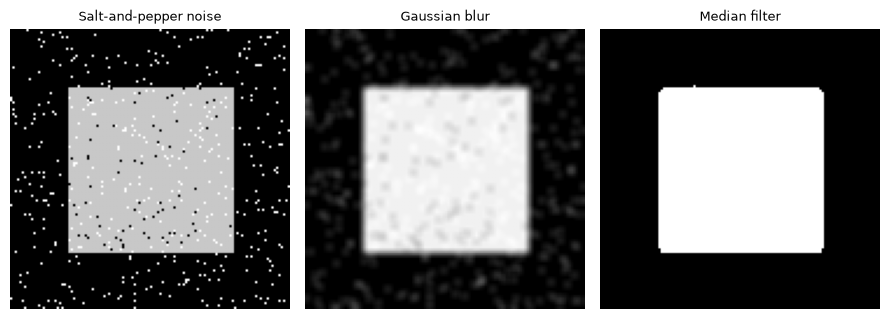
\includegraphics[width=0.9\textwidth]{figures/lesson14_fig01.png}
\caption{Gaussian blur smears each corrupted pixel's extreme value into its neighbors, leaving faint speckle everywhere. The median filter simply outvotes an isolated bad pixel with its many good neighbors, removing nearly all of the noise while keeping edges sharp.}
\label{fig:l14-1}
\end{figure}

\section{Min and max filters: grayscale erosion and dilation}

Chapter~\ref{ch:lesson03} introduced erosion and dilation on \emph{binary} images. On a \textbf{grayscale} image, they generalize naturally: erosion replaces each pixel with the \textbf{minimum} value in its neighborhood, and dilation with the \textbf{maximum}. Both are nonlinear (not a weighted sum), and both are edge-preserving in a different way than blurring --- they shift edges rather than blurring them.

\begin{lstlisting}
def min_filter(image, ksize):
    r = ksize // 2
    padded = cv2.copyMakeBorder(image, r, r, r, r, cv2.BORDER_REPLICATE)
    out = np.zeros_like(image)
    for i in range(image.shape[0]):
        for j in range(image.shape[1]):
            out[i, j] = padded[i:i+ksize, j:j+ksize].min()
    return out
\end{lstlisting}

A from-scratch min filter matches \code{cv2.erode} with a $3\times3$ all-ones kernel exactly, confirming that grayscale erosion really is just a sliding-window minimum.

\section{The problem linear blur can't solve: smoothing without crossing edges}

Gaussian blur treats every neighbor equally regardless of how different its value is --- that's exactly what makes it blur across edges. The \textbf{bilateral filter} fixes this by weighting each neighbor by \emph{two} factors: how close it is spatially (like a Gaussian blur) \textbf{and} how similar its intensity is to the center pixel:
\begin{equation}
I'(p) = \frac{1}{W_p}\sum_{q \in N(p)} G_{\sigma_s}(\|p - q\|) \cdot G_{\sigma_r}(|I(p) - I(q)|) \cdot I(q),
\end{equation}
where $W_p$ normalizes the weights to sum to 1. Neighbors that are spatially close \emph{and} have similar intensity get high weight (smoothed together); neighbors that are spatially close but have very different intensity (i.e.\ on the other side of an edge) get down-weighted almost to zero, so the edge survives.

\begin{lstlisting}
def bilateral_filter(image, radius, sigma_spatial, sigma_range):
    image_f = image.astype(np.float64)
    ys, xs = np.mgrid[-radius:radius+1, -radius:radius+1]
    spatial_weight = np.exp(-(xs**2 + ys**2) / (2 * sigma_spatial**2))
    padded = cv2.copyMakeBorder(image_f, radius, radius, radius, radius, cv2.BORDER_REFLECT101)
    out = np.zeros_like(image_f)
    for i in range(image.shape[0]):
        for j in range(image.shape[1]):
            patch = padded[i:i+2*radius+1, j:j+2*radius+1]
            range_weight = np.exp(-(patch - image_f[i, j])**2 / (2 * sigma_range**2))
            weight = spatial_weight * range_weight
            out[i, j] = (weight * patch).sum() / weight.sum()
    return out
\end{lstlisting}

\code{cv2.bilateralFilter} uses the same idea with some internal approximations for speed, so a close but not pixel-exact match is expected: max absolute difference is $3.40$ gray levels, mean absolute difference $0.56$.

\subsection*{Edge preservation, side by side}

The real comparison that matters: on a noisy step edge, does the filter smooth the noise while keeping the edge sharp, or does it blur the edge along with the noise? Figure~\ref{fig:l14-2} answers this directly.

\begin{figure}[h]
\centering
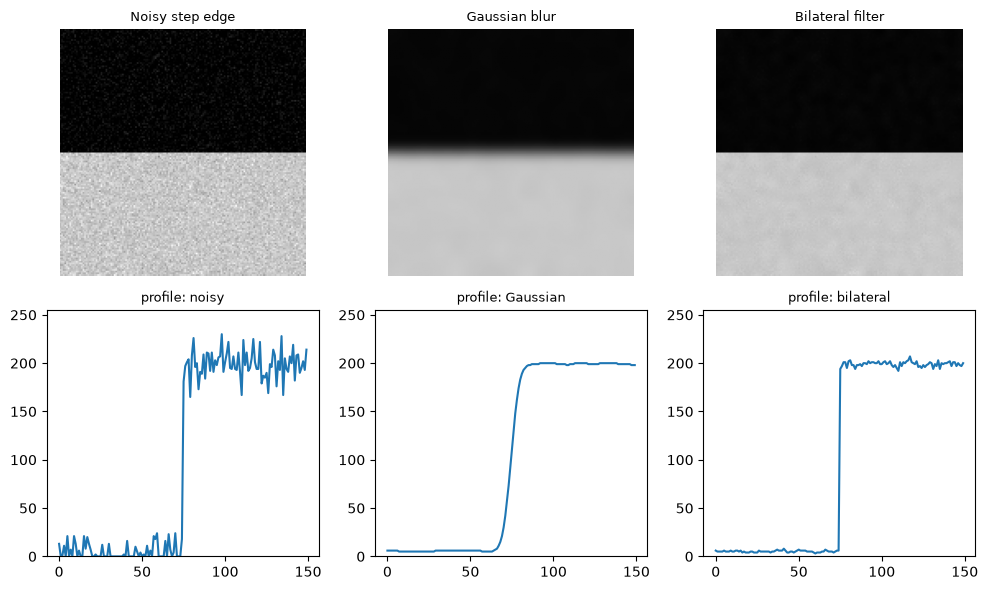
\includegraphics[width=0.95\textwidth]{figures/lesson14_fig02.png}
\caption{Top: a noisy step edge, Gaussian-blurred, and bilateral-filtered. Bottom: intensity profiles along a column crossing the edge. The Gaussian-blurred profile ramps gradually across many rows --- the edge has been visibly softened. The bilateral-filtered profile stays flat on each side (noise removed) but still jumps sharply at the true edge --- it survived because pixels across the boundary were too different in intensity to be averaged together, no matter how spatially close they were.}
\label{fig:l14-2}
\end{figure}

\subsection*{Exercises}
\begin{enumerate}
  \item Apply a median filter (instead of Gaussian or bilateral) to the noisy step edge and add its profile to the comparison. How does it compare to the bilateral filter at preserving the edge?
  \item In \code{bilateral\_filter}, set \code{sigma\_range} very large (e.g.\ 1000). What should this reduce to, and does your result confirm it?
  \item Bilateral filtering is much slower than Gaussian blur because the weights must be recomputed at every pixel (they depend on local intensity, not just position). Time the from-scratch \code{bilateral\_filter} against \code{cv2.bilateralFilter} on a $100\times100$ image with \code{\%timeit}, and describe in words what OpenCV's implementation likely does differently to be faster.
\end{enumerate}

\vfill
\fullcode{lesson14}{lesson14_nonlinear_filters}
